%-*-latex-*-
\sectionthree{Linear recursive runtime}
\begin{python0}
from solutions import *; clear()
\end{python0}

So you see that when you measure the runtime of an algorithm
like our Fibonacci function implemented with linear recursion
will give you a runtime function that looks rather similar.
So the next step is to convert the runtime function
to a \textit{non-recursive} closed form.

Before I show you the closed form for the runtime of Fibonacci, let's just get a feel the
such runtime functions by calculating with one.
It turns out that it's pretty bad.

Suppose I need to solve the problem of computing this
function (it's somewhat like my Fibonacci).
Note that $g(n)$ is defined by linear recursion.
\begin{align*}
g(n) = 
\begin{cases}
1                     & \text{ if $n = 0$} \\
3                     & \text{ if $n = 1$} \\
2g(n - 1) + 3g(n - 2) & \text{ if $n \geq 2$}
\end{cases}
\end{align*}
Suppose I choose to write my algorithm like this:
\begin{Verbatim}[frame=single,fontsize=\footnotesize]
def g(n):
    if n == 0: 
        return 1
    elif n == 1:
        return 3
    else:
        return 2 * g(n - 1) + 3 * g(n - 2)
\end{Verbatim}
You know that the runtime function would be like this:
\[
T(n) = 
\begin{cases}
A                     & \text{if $n = 0, 1$} \\
T(n-1) + T(n-2) + B & \text{if $n > 1$}
\end{cases}
\]
for some constants $A$ and $B$.
Later I'll show you now to compute an approximation (in the big-O sense)
for $T(n)$.
For now, suppose we compute $g(5)$ using the above 
program, compute like what a program would, executing one statement
or one operation at a time.
This is what you would see:

\begin{align*}
g(5)
&= 2g(4) + 3g(3) \\
&= 2(2g(3) + 3g(2)) + 3g(3) \\
&= 2(2(2g(2) + 3g(1)) + 3g(2)) + 3g(3) \\
&= 2(2(2(2g(1) + 3g(0)) + 3g(1)) + 3g(2)) + 3g(3) \\
&= 2(2(2(2(3) + 3g(0)) + 3g(1)) + 3g(2)) + 3g(3) \\
&= 2(2(2(6 + 3g(0)) + 3g(1)) + 3g(2)) + 3g(3) \\
&= 2(2(2(6 + 3(1)) + 3g(1)) + 3g(2)) + 3g(3) \\
&= 2(2(2(6 + 3) + 3g(1)) + 3g(2)) + 3g(3) \\
&= 2(2(2(9) + 3g(1)) + 3g(2)) + 3g(3) \\
&= 2(2(18 + 3g(1)) + 3g(2)) + 3g(3) \\
&= 2(2(18 + 3(3)) + 3g(2)) + 3g(3) \\
&= 2(2(18 + 9) + 3g(2)) + 3g(3) \\
&= 2(2(27) + 3g(2)) + 3g(3) \\
&= 2(54 + 3g(2)) + 3g(3) & & \text{will this ever end?!?} \\
&= 2(54 + 3(2g(1) + 3g(0))) + 3g(3) \\
&= 2(54 + 3(2(3) + 3g(0))) + 3g(3) \\
&= 2(54 + 3(6 + 3g(0))) + 3g(3) \\
&= 2(54 + 3(6 + 3(1))) + 3g(3) \\
&= 2(54 + 3(6 + 3)) + 3g(3) \\
&= 2(54 + 3(9)) + 3g(3) \\
&= 2(54 + 27) + 3g(3) \\
&= 2(81) + 3g(3) \\
&= 162 + 3g(3) \\
&= 162 + 3(2g(2) + 3g(1)) & & \text{ ... oh no ... here we go again ...}\\
&= 162 + 3(2(2g(1) + 3g(0)) + 3g(1)) \\
&= 162 + 3(2(2(3) + 3g(0)) + 3g(1)) \\
&= 162 + 3(2(6 + 3g(0)) + 3g(1)) \\
&= 162 + 3(2(6 + 3(1)) + 3g(1)) \\
&= 162 + 3(2(6 + 3) + 3g(1)) \\
&= 162 + 3(2(9) + 3g(1)) \\
&= 162 + 3(18 + 3g(1)) \\
&= 162 + 3(18 + 3(3)) \\
&= 162 + 3(18 + 9) \\
&= 162 + 3(27) \\
&= 162 + 81 \\
&= 243 & & \text{PHEW!!!}
\end{align*}

\begin{ex}
  Show that if \verb!g(n)! is the following
\begin{Verbatim}[frame=single,fontsize=\footnotesize]
def g(n):
    if n == 0: 
        return 1
    elif n == 1:
        return 3
    else:
        return 2 * g(n - 1) + 3 * g(n - 2)
\end{Verbatim}
Then the runtime is $T(n) = O(2^n)$. (This is the not best big-O.)
What is the space complexity?
\end{ex}

\begin{ex}
  Let
\begin{Verbatim}[frame=single,fontsize=\footnotesize]
def h(n):
    if n == 0: 
        return 1
    elif n == 1:
        return 2
    elif n == 2:
        return 42
    else:
        return 7 * h(n - 1) - 3 * h(n - 2) + 4 * h(n - 3)
\end{Verbatim}
What is a big-O of $T(n)$ for \verb!h(n)!?
What is the space complexity?
\end{ex}


So the execution of $g(5)$ using the above algorithm
seems to indicate that $T(5)$ is huge.
You can see even from this simple simulation that the main
problem is that many function calls were actually repeats.
For instance go ahead and count the number of times
$g(2)$ was executed in the above.

It turns out that except for recursion like this:
\begin{Verbatim}[frame=single,fontsize=\footnotesize]
def h(n):
    if n == 0:
        return 42
    else:
        return 7 * h(n - 1) + n
\end{Verbatim}
where in the recursive part only \textit{one} recursive function call was made,
most cases will usually be extremely bad, as in exponential bad.

It turns out that in general if you have a numeric recursive function
like
\[
T(n) = aT(n - 1) + bT(n - 2) + c
\]
where $a$, $b$, and $c$ are constants,
you can always compute a nice formula for $T(n)$.
A \lq\lq nice'' formula for $T(n)$ that does \textit{not} depend on 
$T(i)$ for smaller $i$ but only on $n$, i.e.,
you can compute a closed form formula for $T(n)$.

In fact more generally there are extremely powerful 
tools to compute an \textit{exact} closed form for more complicated
recursion such as 
\[
T(n) = n^2 T(n-1) + (1 + n) T(n - 2) + \frac{2}{3}n^2 - 1 
\]
But I'll stick to the simple case of
\[
T(n) = aT(n - 1) + bT(n - 2) + c
\]
where $a,b,c$ are constants.

Although there are techniques to compute exact closed forms for $T(n)$,
remember that we only need the big-O of $T(n)$.

For the case of a recursive function such as 
\begin{Verbatim}[frame=single,fontsize=\footnotesize]
def g(n):
    if n == 0: 
        return 1
    elif n == 1:
        return 3
    else:
        return 2 * g(n - 1) + 3 * g(n - 2)
\end{Verbatim}
which has a runtime $T(n)$ satisfying
\[
T(n) = T(n - 1) + T(n - 2) + A
\]
where $A$ is a constant, a rough approximation (using the method
in an earlier section) the runtime is
\[
T(n) = O(2^n)
\]
i.e., exponential.
Which means the runtime is bad.
How bad? What exactly is \lq\lq exponential bad"?
You can use the fibonacci function as an example:
\begin{Verbatim}[frame=single,fontsize=\footnotesize]
def fib(n):
    if n == 0: 
        return 1
    elif n == 1:
        return 1
    else:
        return fib(n - 1) + fib(n - 2)
\end{Verbatim}
and print \verb!fib(n)! for \verb!n = 0, 1, 2, ..., 100!.
Remember we did this before in CISS245.
It will grind to a halt before hitting \verb!60!.

In the above, instead of $O(2^n)$, we can be more precise.

First, you ignore the constant $c$ in
\[
T(n) = aT(n - 1) + bT(n - 2) + c \tag{1}
\]
and look at this recursion instead:
\[
T^{(h)}(n) = aT^{(h)}(n - 1) + bT^{(h)}(n - 2) \tag{2}
\]
This is called the \defone{homogeneous part} of $T(n)$.
You need to know that $T^{(h)}(n)$ must have a solution
roughly of the form
\[
T^{(h)}(n) = r^n
\]
where $r$ is a constant.
(Take this on faith for now -- the justification will be
provided in MATH325.)
The immediate goal now is to compute $r$.
You substitute this into (2) to get
\[
r^n = ar^{n-1} + br^{n-2}
\]
You cross out $r^{n - 2}$ to get
\[
r^2 = ar + b
\]
i.e., a quadratic equation.
This then allows you to solve for $r$.

Let's try this technique on our
\[
T(n) = T(n - 1) + T(n - 2) + d
\]
The homogeneous of of this equation is
\[
T^{(h)}(n) = T^{(h)}(n - 1) + T^{(h)}(n - 2)
\]
Let $T^{(h)}(n) = r^n$ and substitute it into
\[
T^{(h)}(n) = T^{(h)}(n - 1) + T^{(h)}(n - 2)
\]
to get
\[
r^n = r^{n - 1} + r^{n - 2}
\]
Cross out $r^{n - 2}$ to get
\[
r^2 = r + 1
\]
which gives us the quadratic
\[
r^2 - r - 1 = 0
\]
Using the quadratic polynomial root formula you get
\[
r = \frac{-(-1) \pm \sqrt{(-1)^2 - 4(1)(-1)} }{2}
\]
which gives us
\[
r = \frac{1 \pm \sqrt{5}}{2}
\]
Let 
\[
r_1 = \frac{1 + \sqrt{5} }{2} 
\]
(... this is the one that is about 1.618)
and 
\[
r_2 = \frac{1 - \sqrt{5} }{2}
\]
Then you know that if the recurrence relation on $T^{(h)}(n)$ is
\[
T^{(h)}(n) = T^{(h)}(n - 1) + T^{(h)}(n - 2)
\]
then $T^{(h)}(n)$ must have the form
\[
T^{(h)}(n) = \alpha \cdot r_1^n + \beta \cdot r_2^n
\]
where $\alpha, \beta$ are constants.

This is the closed form for $T^{(h)}(n)$.
But what about $T(n)$? Remember that
\[
T(n) = T^{(h)}(n) + d
\]
The next thing you need to know is that
if $r_1$ and $r_2$ are both $1$, then
\[
\]

Now, $|r_2| = 0.618...$ whereas $r_1 = 1.618...$.
Therefore
\[
T^{(h)}(n) = \alpha \cdot r_1^n + \beta \cdot r_2^n = O(r_1^n)
\]
which means that the algorithm has exponential runtime
but the base of the exponential runtime is $1.618...$ instead of $2$.
Note that $2^n$ climbs much faster than $1.618^n$.
That's because
\[
\frac{2^n}{1.618^n} = 1.236...^n
\]
and $1.236...^n$ grows toward infinity as $n$ grows unboundedly
since $1.236 > 1$.

Note that at the stage where you solve for $r$ in 
the quadratic equation in $r$:
\[
r^2 = ar + b \tag{*}
\]
you will have \textit{three} cases: $(*)$ has
\begin{align*}
\text{Case 1:} & \ \text{two distinct real roots} \\
\text{Case 2:} & \ \text{two distinct complex (and nonreal) roots} \\
\text{Case 3:} & \ \text{two roots with the same real value}
\end{align*}
The Fibonacci case of 
\[
r^2 = r + 1
\]
gives us two distinct real roots.

For case (a) and (b) above, the $T(n)$ is just
\[
T(n) = \alpha r_1^n + \beta r_2^n
\]
(Unfortunately for case (b) you would have to use complex
numbers.)
For the third case where there is one value $r_1$ for both roots,
the closed form becomes
\[
T(n) = \alpha r_1^n + \beta nr_1^n
\]
so in this case
\[
T(n) = O(nr_1^n)
\]
Of course as for the specific big-O class, you have to 
compute the exact root values.

[EXERCISES]

%\newpage
%\subsection*{Solutions}
%
\newpage
\section*{Solutions}
Solution to Exercise \ref{ex:dfa0}\labeltext{}{sol:dfa0}.

\tinysidebar{\debug{exercises/{dfa0/answer.tex}}}

    Solution not provided.
    

\newpage

Solution to Exercise \ref{ex:dfa1}\labeltext{}{sol:dfa1}.

\tinysidebar{\debug{exercises/{dfa1/answer.tex}}}
  The ID computation is
  \begin{align*}
    (q_0, aba)
    &\vdash (\delta(q_0, a), ba) = (q_0, ba) \\ 
    &\vdash (\delta(q_0, b), a) = (q_1, a) \\
    &\vdash (\delta(q_1, a), \ep) = (q_0, \ep)
  \end{align*}
  $q_0$ is not an accept state. Therefore $aba$ is not accepted.


\newpage

Solution to Exercise \ref{ex:dfa4}\labeltext{}{sol:dfa4}.

\tinysidebar{\debug{exercises/{dfa4/answer.tex}}}

    Solution not provided.
    

\newpage

Solution to Exercise \ref{ex:dfa5}\labeltext{}{sol:dfa5}.

\tinysidebar{\debug{exercises/{dfa5/answer.tex}}}

    Solution not provided.
    

\newpage

Solution to Exercise \ref{ex:implementing-a-single-dfa0}\labeltext{}{sol:implementing-a-single-dfa0}.

\tinysidebar{\debug{exercises/{implementing-a-single-dfa0/answer.tex}}}

    Solution not provided.
    

\newpage

Solution to Exercise \ref{ex:nfastatediag0}\labeltext{}{sol:nfastatediag0}.

\tinysidebar{\debug{exercises/{nfastatediag0/answer.tex}}}

    Solution not provided.
    

\newpage

Solution to Exercise \ref{ex:nfastatediag1}\labeltext{}{sol:nfastatediag1}.

\tinysidebar{\debug{exercises/{nfastatediag1/answer.tex}}}

    Solution not provided.
    

\newpage

Solution to Exercise \ref{ex:nfastatediag2}\labeltext{}{sol:nfastatediag2}.

\tinysidebar{\debug{exercises/{nfastatediag2/answer.tex}}}

    Solution not provided.
    

\newpage

Solution to Exercise \ref{ex:nfastatediag3}\labeltext{}{sol:nfastatediag3}.

\tinysidebar{\debug{exercises/{nfastatediag3/answer.tex}}}

    Solution not provided.
    

\newpage

Solution to Exercise \ref{ex:nfastatediag4}\labeltext{}{sol:nfastatediag4}.

\tinysidebar{\debug{exercises/{nfastatediag4/answer.tex}}}

    Solution not provided.
    

\newpage

Solution to Exercise \ref{ex:nfastatediag5}\labeltext{}{sol:nfastatediag5}.

\tinysidebar{\debug{exercises/{nfastatediag5/answer.tex}}}

    Solution not provided.
    

\newpage

Solution to Exercise \ref{ex:nfastatediag6}\labeltext{}{sol:nfastatediag6}.

\tinysidebar{\debug{exercises/{nfastatediag6/answer.tex}}}

    Solution not provided.
    

\newpage

Solution to Exercise \ref{ex:nfastatediag7}\labeltext{}{sol:nfastatediag7}.

\tinysidebar{\debug{exercises/{nfastatediag7/answer.tex}}}

    Solution not provided.
    

\newpage

Solution to Exercise \ref{ex:nfastatediag8}\labeltext{}{sol:nfastatediag8}.

\tinysidebar{\debug{exercises/{nfastatediag8/answer.tex}}}

    Solution not provided.
    

\newpage

Solution to Exercise \ref{ex:nfastatediag9}\labeltext{}{sol:nfastatediag9}.

\tinysidebar{\debug{exercises/{nfastatediag9/answer.tex}}}

    Solution not provided.
    

\newpage

Solution to Exercise \ref{ex:nfastatediag10}\labeltext{}{sol:nfastatediag10}.

\tinysidebar{\debug{exercises/{nfastatediag10/answer.tex}}}

    Solution not provided.
    

\newpage

Solution to Exercise \ref{ex:nfastatediag11}\labeltext{}{sol:nfastatediag11}.

\tinysidebar{\debug{exercises/{nfastatediag11/answer.tex}}}

    Solution not provided.
    

\newpage

Solution to Exercise \ref{ex:nfastatediag12}\labeltext{}{sol:nfastatediag12}.

\tinysidebar{\debug{exercises/{nfastatediag12/answer.tex}}}

    Solution not provided.
    

\newpage

Solution to Exercise \ref{ex:nfastatediag13}\labeltext{}{sol:nfastatediag13}.

\tinysidebar{\debug{exercises/{nfastatediag13/answer.tex}}}

    Solution not provided.
    

\newpage

Solution to Exercise \ref{ex:nfa0}\labeltext{}{sol:nfa0}.

\tinysidebar{\debug{exercises/{nfa0/answer.tex}}}
The formal definition of this NFA is $(\Sigma, Q, q_0, \delta, F)$ where
\begin{tightlist}
\li $\Sigma = \{a,b\}$
\li $Q = \{q_0\}$
\li $\delta$ is the function
\[
\delta : Q \times \Sigma_\epsilon \rightarrow P(Q)
\]
given by
\begin{align*}
  \delta(q_0, \epsilon) &= \{\} \\
  \delta(q_0, a) &= \{\} \\
  \delta(q_0, b) &= \{\} 
\end{align*}
\end{tightlist}


\newpage

Solution to Exercise \ref{ex:nfa1}\labeltext{}{sol:nfa1}.

\tinysidebar{\debug{exercises/{nfa1/answer.tex}}}

    Solution not provided.
    

\newpage

Solution to Exercise \ref{ex:nfa2}\labeltext{}{sol:nfa2}.

\tinysidebar{\debug{exercises/{nfa2/answer.tex}}}

    Solution not provided.
    

\newpage

Solution to Exercise \ref{ex:nfa3}\labeltext{}{sol:nfa3}.

\tinysidebar{\debug{exercises/{nfa3/answer.tex}}}

    Solution not provided.
    

\newpage

Solution to Exercise \ref{ex:nfa4}\labeltext{}{sol:nfa4}.

\tinysidebar{\debug{exercises/{nfa4/answer.tex}}}

    Solution not provided.
    

\newpage

Solution to Exercise \ref{ex:nfa5}\labeltext{}{sol:nfa5}.

\tinysidebar{\debug{exercises/{nfa5/answer.tex}}}

    Solution not provided.
    

\newpage

Solution to Exercise \ref{ex:dfa-as-powerful-as-nfa0}\labeltext{}{sol:dfa-as-powerful-as-nfa0}.

\tinysidebar{\debug{exercises/{dfa-as-powerful-as-nfa0/answer.tex}}}
Here's the solution.
Let $\delta$ denote the transition function of $N$.
Note that 
\begin{align*}
  \delta(q_0, \epsilon) = \{\} \\
  \delta(q_0, a) = \{\} \\
  \delta(q_0, b) = \{\} 
\end{align*}
First of all the states are labeled as all the subsets of $\{q_0\}$.


\begin{center}
\begin{tikzpicture}[>=triangle 60,shorten >=0.5pt,node distance=2cm,auto,initial text=, double distance=2pt]
\node[state] (A) at (  0,  0) {$\{q_0\}$};
\node[state] (B) at (  3,  0) {$\{\}$};

\path[->]

;
\end{tikzpicture}
\end{center}
    


The start state is the $\epsilon$-closure of $\{q_0\}$.
However in $N$, there are no $\epsilon$--transitions out of 
$q_0$.
So the $\epsilon$-closure of $\{q_0\}$ is in fact $\{q_0\}$, i.e.
$\overline{\{q_0\}} = \{q_0\}$
The $\DFA$ is now this:


\begin{longtable}{|r||r|r|r|r|r|}
\hline 
         & $w_1$ & $w_2$ & $w_3$ & $w_4$ & $\ldots$ \\ \hline \hline 
$M_1$    &       &       &       &       &          \\ \hline 
$M_2$    &       &       &       &       &          \\ \hline 
$M_3$    &       &       &       &       &          \\ \hline 
$M_4$    &       &       &       &       &          \\ \hline 
$\ldots$ &       &       &       &       &          \\ \hline 
\end{longtable}
        


Now I will compute the $a$--transition of the state $\{q_0\}$.
Let $\delta^\DFA$ denote the transition function of the $\DFA$
that we're building.
Then
\begin{align*}
\delta( \{q_0, a\} ) 
&= \overline{ \bigcup_{q \in \{q_0\}} \delta(q, a)} \\
&= \overline{ \delta(q_0, a) } \\
&= \overline{ \emptyset } \\
&= \emptyset
\end{align*}
The (incomplete) $\DFA$ now looks like this:


\begin{longtable}{|r||r|r|r|r|r|}
\hline 
         & $w_1$ & $w_2$ & $w_3$ & $w_4$ & $\ldots$ \\ \hline \hline 
$M_1$    & 0     & 0     & 1     & 0     & ...      \\ \hline 
$M_2$    & 1     & 0     & 1     & 1     & ...      \\ \hline 
$M_3$    & 0     & 1     & 1     & 1     & ...      \\ \hline 
$M_4$    & 1     & 0     & 1     & 1     & ...      \\ \hline 
$\ldots$ &       &       &       &       &          \\ \hline 
\end{longtable}
        


Using the same reasoning we have

\begin{center}
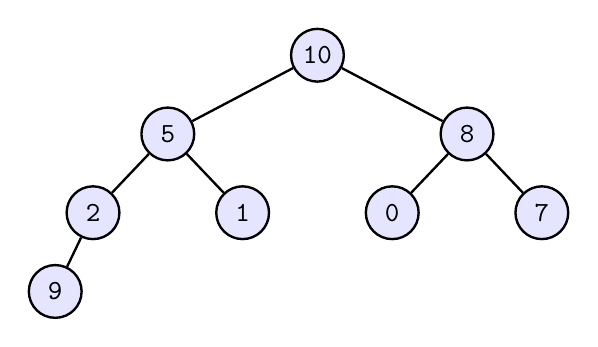
\begin{tikzpicture}

\fill[blue!10] (0.0, 0.0) circle (0.35);
\node [line width=0.03cm,black,minimum size=0.6699999999999999cm,draw,circle] at (0.0,0.0)(10){};\draw (0.0, 0.0) node[color=black] {\texttt{10}};
\fill[blue!10] (-1.9, -1.0) circle (0.35);
\node [line width=0.03cm,black,minimum size=0.6699999999999999cm,draw,circle] at (-1.9,-1.0)(5){};\draw (-1.9, -1.0) node[color=black] {\texttt{5}};
\fill[blue!10] (1.9, -1.0) circle (0.35);
\node [line width=0.03cm,black,minimum size=0.6699999999999999cm,draw,circle] at (1.9,-1.0)(8){};\draw (1.9, -1.0) node[color=black] {\texttt{8}};
\fill[blue!10] (-2.85, -2.0) circle (0.35);
\node [line width=0.03cm,black,minimum size=0.6699999999999999cm,draw,circle] at (-2.85,-2.0)(2){};\draw (-2.85, -2.0) node[color=black] {\texttt{2}};
\fill[blue!10] (-0.95, -2.0) circle (0.35);
\node [line width=0.03cm,black,minimum size=0.6699999999999999cm,draw,circle] at (-0.95,-2.0)(1){};\draw (-0.95, -2.0) node[color=black] {\texttt{1}};
\fill[blue!10] (0.95, -2.0) circle (0.35);
\node [line width=0.03cm,black,minimum size=0.6699999999999999cm,draw,circle] at (0.95,-2.0)(0){};\draw (0.95, -2.0) node[color=black] {\texttt{0}};
\fill[blue!10] (2.85, -2.0) circle (0.35);
\node [line width=0.03cm,black,minimum size=0.6699999999999999cm,draw,circle] at (2.85,-2.0)(7){};\draw (2.85, -2.0) node[color=black] {\texttt{7}};
\fill[blue!10] (-3.33, -3.0) circle (0.35);
\node [line width=0.03cm,black,minimum size=0.6699999999999999cm,draw,circle] at (-3.33,-3.0)(9){};\draw (-3.33, -3.0) node[color=black] {\texttt{9}};\draw[line width=0.03cm,black] (10) to  (5);
\draw[line width=0.03cm,black] (10) to  (8);
\draw[line width=0.03cm,black] (5) to  (2);
\draw[line width=0.03cm,black] (5) to  (1);
\draw[line width=0.03cm,black] (8) to  (0);
\draw[line width=0.03cm,black] (8) to  (7);
\draw[line width=0.03cm,black] (2) to  (9);
\end{tikzpicture}

\end{center}



It's easy to see that in the DFA, the $a$--
and $b$--transitions from the state $\{\}$ goes back to itself.
Therefore the completed DFA is this:


\begin{center}
\begin{tikzpicture}[>=triangle 60,shorten >=0.5pt,node distance=2cm,auto,initial text=, double distance=2pt]
\node[state,initial] (A) at (  0,  0) {$\{q_0\}$};
\node[state] (B) at (  3,  0) {$\{\}$};

\path[->]
(A) edge [bend left=0,pos=0.5,above] node {$a,b$} (B)
(B) edge [loop above] node {$a,b$} ()

;
\end{tikzpicture}
\end{center}
    



\newpage

Solution to Exercise \ref{ex:dfa-as-powerful-as-nfa1}\labeltext{}{sol:dfa-as-powerful-as-nfa1}.

\tinysidebar{\debug{exercises/{dfa-as-powerful-as-nfa1/answer.tex}}}

    Solution not provided.
    

\newpage

Solution to Exercise \ref{ex:dfa-as-powerful-as-nfa2}\labeltext{}{sol:dfa-as-powerful-as-nfa2}.

\tinysidebar{\debug{exercises/{dfa-as-powerful-as-nfa2/answer.tex}}}

    Solution not provided.
    

\newpage

Solution to Exercise \ref{ex:dfa-as-powerful-as-nfa3}\labeltext{}{sol:dfa-as-powerful-as-nfa3}.

\tinysidebar{\debug{exercises/{dfa-as-powerful-as-nfa3/answer.tex}}}

    Solution not provided.
    

\newpage

Solution to Exercise \ref{ex:dfa-as-powerful-as-nfa4}\labeltext{}{sol:dfa-as-powerful-as-nfa4}.

\tinysidebar{\debug{exercises/{dfa-as-powerful-as-nfa4/answer.tex}}}

    Solution not provided.
    

\newpage

Solution to Exercise \ref{ex:closure0}\labeltext{}{sol:closure0}.

\tinysidebar{\debug{exercises/{closure0/answer.tex}}}

    Solution not provided.
    

\newpage

Solution to Exercise \ref{ex:closure1}\labeltext{}{sol:closure1}.

\tinysidebar{\debug{exercises/{closure1/answer.tex}}}

    Solution not provided.
    

\newpage

Solution to Exercise \ref{ex:closure2}\labeltext{}{sol:closure2}.

\tinysidebar{\debug{exercises/{closure2/answer.tex}}}

    Solution not provided.
    

\newpage

Solution to Exercise \ref{ex:closure3}\labeltext{}{sol:closure3}.

\tinysidebar{\debug{exercises/{closure3/answer.tex}}}

    Solution not provided.
    

\newpage

Solution to Exercise \ref{ex:closure4}\labeltext{}{sol:closure4}.

\tinysidebar{\debug{exercises/{closure4/answer.tex}}}

    Solution not provided.
    

\newpage

Solution to Exercise \ref{ex:closure5}\labeltext{}{sol:closure5}.

\tinysidebar{\debug{exercises/{closure5/answer.tex}}}

    Solution not provided.
    

\newpage

Solution to Exercise \ref{ex:closure6}\labeltext{}{sol:closure6}.

\tinysidebar{\debug{exercises/{closure6/answer.tex}}}

    Solution not provided.
    

\newpage

Solution to Exercise \ref{ex:closure7}\labeltext{}{sol:closure7}.

\tinysidebar{\debug{exercises/{closure7/answer.tex}}}

    Solution not provided.
    

\newpage

Solution to Exercise \ref{ex:closure8}\labeltext{}{sol:closure8}.

\tinysidebar{\debug{exercises/{closure8/answer.tex}}}

    Solution not provided.
    

\newpage

Solution to Exercise \ref{ex:closure9}\labeltext{}{sol:closure9}.

\tinysidebar{\debug{exercises/{closure9/answer.tex}}}

    Solution not provided.
    

\newpage

Solution to Exercise \ref{ex:closure10}\labeltext{}{sol:closure10}.

\tinysidebar{\debug{exercises/{closure10/answer.tex}}}

    Solution not provided.
    

\newpage

Solution to Exercise \ref{ex:closure11}\labeltext{}{sol:closure11}.

\tinysidebar{\debug{exercises/{closure11/answer.tex}}}

    Solution not provided.
    

\newpage

Solution to Exercise \ref{ex:closure12}\labeltext{}{sol:closure12}.

\tinysidebar{\debug{exercises/{closure12/answer.tex}}}

    Solution not provided.
    

